144. \begin{figure}[ht!]
\center{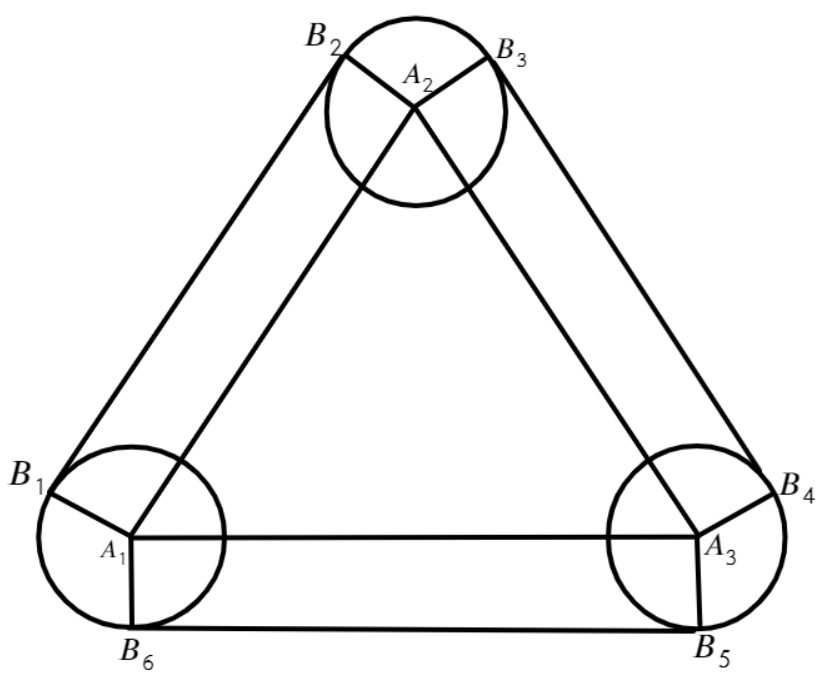
\includegraphics[scale=0.35]{g9-144a.png}}
\end{figure}\\
Искомую площадь составляют три прямоугольника $A_1B_1B_2A_2,\ A_2B_3B_4A_3$ и $A_3B_5B_6A_1,$ имеющие размеры $400\text{ м}\times100\text{ м}$ и три сектора с углом $120^\circ$ $A_1B_1B_6,\ A_2B_2B_3$ и $A_3B_4B_5,$ вместе составляющие полный круг с радиусом 100 м. Значит, простреливаемая снаружи крепости площадь равна $100\cdot400\cdot3+\pi\cdot100^2=120000+10000\pi=10000(\pi+12)\text{ м}^2.$\\
б) \begin{figure}[ht!]
\center{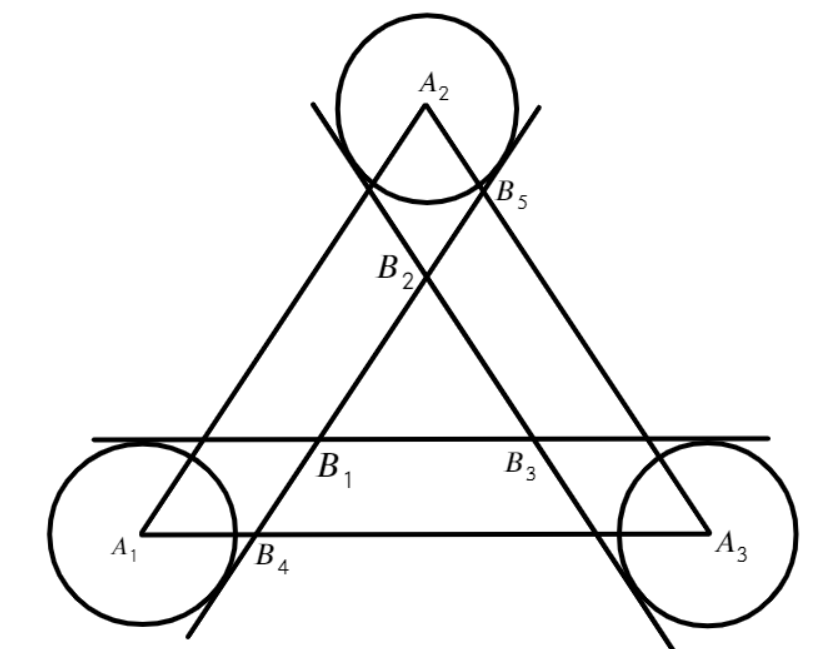
\includegraphics[scale=0.35]{g9-144b.png}}
\end{figure}\\
Искомая площадь --- это разность площадей правильных треугольников $A_1A_2A_3$ и $B_1B_2B_3.$ Для нахождения стороны треугольника $B_1B_2B_3$ рассмотрим трапецию $A_1A_2B_5B_4.$ Её основание $A_1A_2$ равно 400 м, а высота равна 100 м, углы при основании равны $60^\circ.$ Если провести высоты $B_4H_1$ и $B_5H_2,$ то  $A_1H_1=A_2H_2=100\ ctg(60^\circ)=100\sqrt{3}$м. Тогда $B_1B_2=H_1H_2=400-200\sqrt{3}=200(2-\sqrt{3}).$ Тогда $S_{\Delta A_1A_2A_3}-S_{\Delta B_1B_2B_3}=\cfrac{\sqrt{3}}{4}\cdot160000-\cfrac{\sqrt{3}}{4}\cdot40000\cdot(4-4\sqrt{3}+3)=
10000\sqrt{3}(4-7+4\sqrt{3})=30000(4-\sqrt{3})\text{ м}^2.$\newpage\noindent
